\chapter{Giới thiệu}
Mạng nơ ron sâu (DNNs) đã đạt hiệu quả rất tốt với các bài toán trong học máy
và trí tuệ nhân tạo như phân loại ảnh, nhận diện giọng nói, dịch máy và trò chơi.
Mặc dù DNNs rất hiệu quả nhưng mốt số nghiên cứu gần đây đã chứng minh DNNs rất 
dễ  "tổn thương" với các mẫu đối thủ (Szegedy et al. 2013; Goodfellow, Shlens, 
and Szegedy 2015). Ví dụ, một hình ảnh với nhiễu được thiết kế cẩn thận có thể
làm cho một DNNs đã được huấn luyện phân loại sai. Tệ hơn nữa, các mẫu đối thủ
được tạo ra hầu như không thể phân biệt được bằng mắt người. 
\begin{figure}[H] % places figure environment here   
    \centering % Centers Graphic
    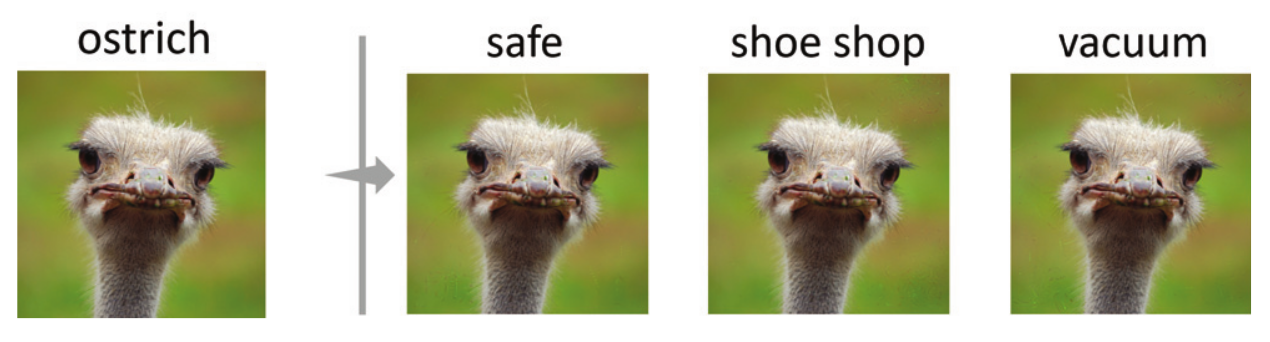
\includegraphics[width=0.8\textwidth]{assets/fig_01.png} 
    \caption{Minh họa trực quan về mẫu đối thủ được sinh bởi EAD. 
    Hình gốc (đà điểu) được lấy từ tập ImageNet. Các mẫu đối thủ bị 
    phân loại sai với mô hình Inception-v3.} % Creates caption underneath graph
    \label{fig:fg_01}
\end{figure}